
    % \begin{minipage}{0.5\textwidth}
%     \centering
%     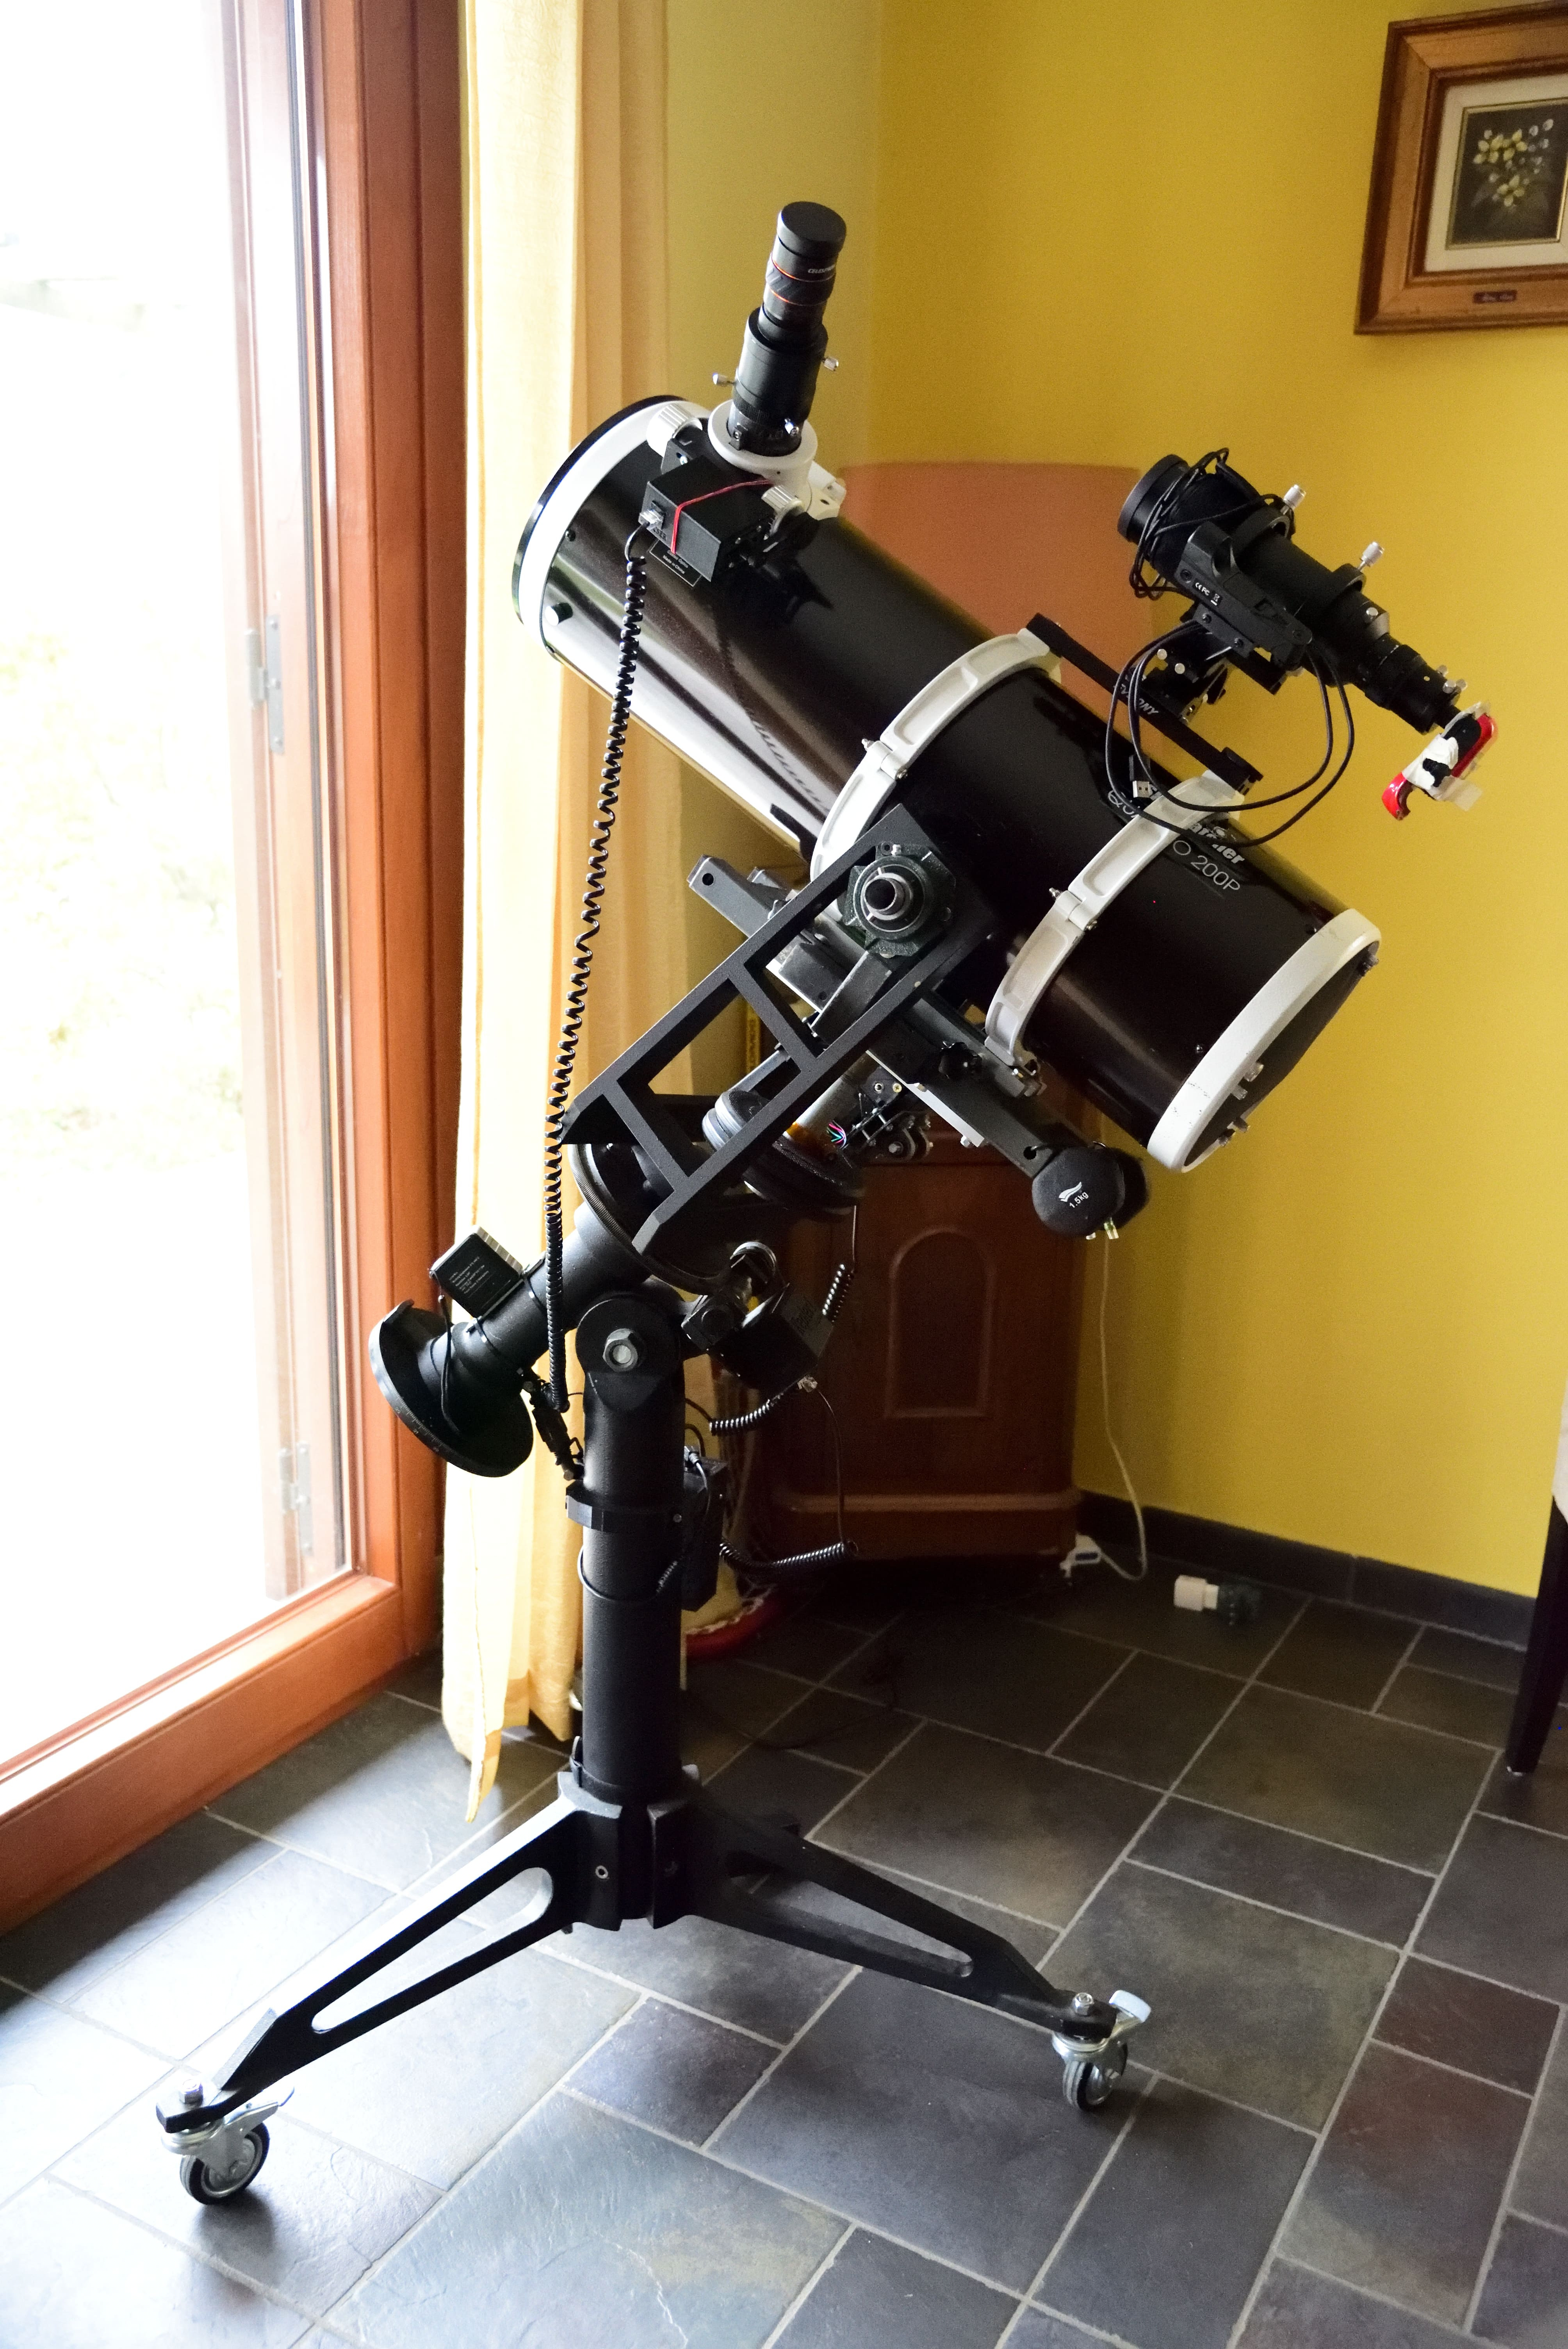
\includegraphics[scale=0.04]{DSC_5264_00001.jpg}
%     \captionof{figure}{Final result: our brand-new telescope.}
% \end{minipage}

\section{Telescope description}
The starting point of the project is of course the telescope.
In our garage, for many years, a 1980 Urania telescope has eaten a lot of dust.
The telescope's mirror resent of years in humidity and temperature jumps in the garage.
In the beginning, we have cleaned the silvered-mirror with soap and water, but the silver still seemed to be a bit compromised.
We do not talk long about this telescope, since we have soon substituted it with a brand-new Skywatcher Quattro.
The latter is placed on the Urania mount, since it is still a nice mount and, in our advice, has still not surpassed robustness.
Indeed, the mount is a very heavy (telescope and mount totally weight 20kg!) equatorial and motorized (still works!) mount.

For our money, but most importantly for our fun and entertainment, we decided to modernize our old telescope.

\subsection{Urania telescope}
We briefly add the specifics of the old Urania telescope, as a sort of respect for many years of honorable work before the deep dark in the garage.
\\
\begin{minipage}{0.5\textwidth}
    \centering
    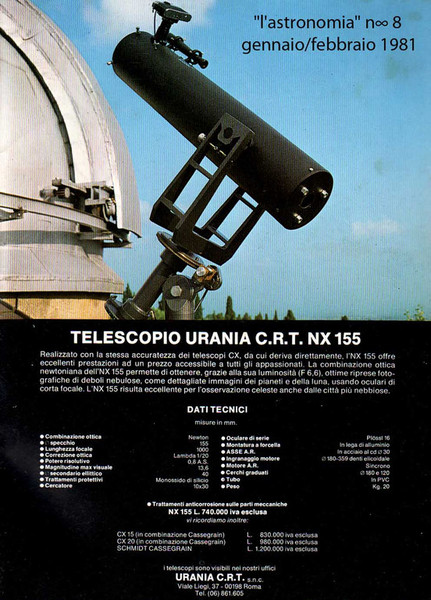
\includegraphics[scale=0.4]{urania_upper.jpg}
    \captionof{figure}{Urania telescope and mount.}
    \label{fig:urania_telescope_mount}
\end{minipage}
\\
The telescope is a Urania C.R.T. NX 155, as the one in figure \ref{fig:urania_telescope_mount}.
\\
\begin{minipage}{0.5\textwidth}
    \centering
    \begin{tabular}{c|c}
        Specific name & value \\
        \hline
        type & reflector \\
        technique & Newton  \\
        material & PVC  \\
        weight (kg) & 10 \\
        aperture (mm) & 155 \\
        focal length (mm) & 1000 \\
        focal & f/6.5 \\
        resolution power & 0.8 \\
        limit magnitude value (mag) & 13.6 \\
        Mirror Treatment & Silica monoxide \\
        \hline
    \end{tabular}
    \captionof{table}{Urania C.R.T. NX 155 specifics.}
\end{minipage}

\subsection{Telescope's mount}
The telescope is place onto an aeronautic Aluminum tripod equatorial mount.
\\
\begin{minipage}{.4\textwidth}
    \begin{tabular}{cc}
        Specific & value \\
        \hline
        weight (kg) & \\
        type & fork \\
        material & Aluminum alloy \\
        RA axis diameter (mm) & 30 \\
        RA axis material & cadmium steel \\
        RA motor & 3W synchronous \\
        \hline
    \end{tabular}
    \captionof{table}{Urania's mount specifics.}
    \label{tab:mount}
\end{minipage}

Starting from the bottom: three pods of 30cm depart from a central post. Each one has a wheel which permits the structure to move freely and then to fix the position using stops.
The central post terminates with the second axis holder at an inclination equal to the Earth's ecliptic \(23.43^{\circ} = 23^{\circ} 26'\).

This axis must be aligned with the Polar star (labelling the North).
In this way, a 3W synchronous motor can follow the sky movement.

Departing from this second axis, a two-arms fork is free to rotate around two degrees-of-freedom defining the right ascension (RA) and the declination (DEC).
The two arms are separated by the distance \(d = 15\)mm which is the Urania telescope aperture.
\subsection{Skywatcher 8P Quattro telescope}
Skywatcher 8P Quattro Newtonian telescope (figure \ref{fig:skywatcher_telescope_mount}) offers an optimal astrophotography performance.
For this reason we have decided to substitute the Urania telescope with this brand-new Skywatcher telescope.
\\
\begin{minipage}{0.5\textwidth}
    \centering
    \begin{tabular}{c|c}
        Specific name & value \\
        \hline
        type & reflector \\
        technique & Newton  \\
        material & Carbon  \\
        weight (kg) & 8.0 \\
        aperture (mm) & 200 \\
        focal length (mm) & 800 \\
        focal & f/4 \\
        resolution power & 0.58 \\
        limit magnitude (mag) & 13.3 \\
        collect light & 820 \\
        magnification & 400 \\
        Mirror Treatment & Aluminum Coating \\
        Focuser & Crayford dual-speed 50.8/31.8 \\
        \hline
    \end{tabular}
    \captionof{table}{Skywatcher 8P Quattro}
    \label{tab_skywatcher_quattro}
\end{minipage}
\\
\begin{minipage}{0.5\textwidth}
    \centering
    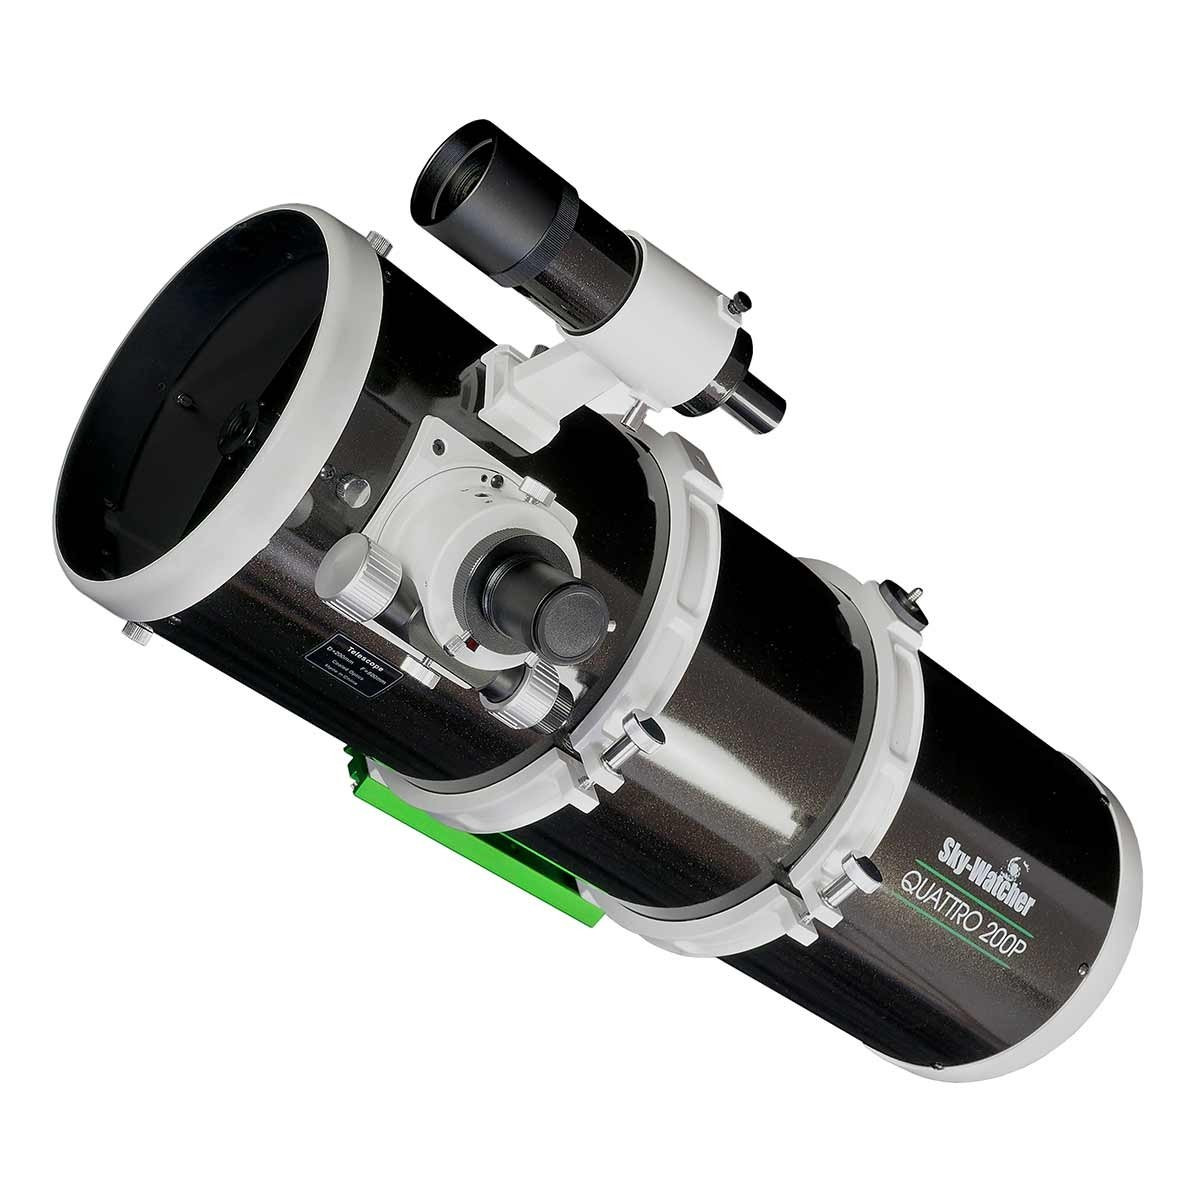
\includegraphics[scale=0.2]{newton-quattro-200-sky-watcher.jpg}
    \captionof{figure}{Skywatcher Quattro telescope.}
    \label{fig:skywatcher_telescope_mount}
\end{minipage}
\\
Since the Skywatcher telescope does not fit in the fork, we have thought to build a "saddle" onto which placing the telescope.
The specifics of this installation are shown in the following section.